\documentclass[english,sort&compress]{elsarticle}

\newcommand{\folder}{/Users/steeve/MA_ZONE/BIBLIO}

% ---------------------------- Packages inclusions.
\usepackage[T1]{fontenc}
\usepackage[utf8]{inputenc}
\usepackage[a4paper]{geometry}
\geometry{verbose}
\usepackage{amsthm,amsmath,amssymb,graphicx,esint,bbm,tabularx}
\usepackage{times}%\usepackage{subfloat}
%\usepackage{subfig}
\usepackage{babel}
%\usepackage{calrsfs}

% ---------------------------- Pour l'impression et user au mieux la page
\textwidth = 18.5cm
\textheight = 26cm
\oddsidemargin = -1.25cm
\evensidemargin = -1.25cm
\topmargin = -2.25cm

% ---------------------------- Textclass specific LaTeX commands.
\theoremstyle{definition}
\newtheorem{defn}{\protect\definitionname}
\theoremstyle{plain}
\newtheorem{prop}{\protect\propositionname}
\theoremstyle{plain}
\newtheorem{thm}{\protect\theoremname}
\providecommand{\definitionname}{Definition}
\providecommand{\propositionname}{Proposition}
\providecommand{\theoremname}{Theorem}


% ---------------------------- User specified LaTeX commands.
\def\d{\mathrm{d}}
\def\dmu{\mathrm{d}\mu}
\def\fD{\mathcal{D}}
\def\Rset{\mathbb{R}}
\def\X{\mathcal{X}}
%\def\x{\chi}
\def\Y{\mathcal{Y}}
\def\un{\mathbbm{1}}
\def\e{\operatorname{e}}
\def\W{\operatorname{W}}
\def\ext{\operatorname{ext}}
\def\sech{\operatorname{sech}}
\def\arsech{\operatorname{arsech}}
\def\argtanh{\operatorname{argtanh}}
%
\newcommand{\Esp}[1]{\mathbb{E}\left[ #1 \right]}
\newcommand{\hypgeom}[2]{\mbox{}_{#1}\hspace{-1pt}F_{#2}}


% ---------------------------- Suppress the footpage
%                              ('preprint submitted to Elsevier' mention)
\makeatletter
\def\ps@pprintTitle{%
  \let\@oddhead\@empty
  \let\@evenhead\@empty
  \def\@oddfoot{\reset@font\hfil\thepage\hfil}
  \let\@evenfoot\@oddfoot
}



% ------------------------ Beginning of the document ------------------------ %
% --------------------------------------------------------------------------- %

\begin{document}


% -------------------------------- Frontpage -------------------------------- %

\title{T'aurais pas une entropie?}
\author{by jfb \& co \date{} }
\begin{abstract}
  Where  we  show  that it  is  possible  to  derive  new entropies  yielding  a
  particular specified  maximum entropy distribution. There  are (probably) many
  errors  --I  hope  not  fundamental  but  is  is  possible;  (certainly  many)
  approximations,   typos,   maths   and   language   mistakes.Suggestions   and
  improvements will be much appreciated.
\end{abstract}

\maketitle


% ---------------------------------- MaxEnt ---------------------------------- %

\section{Maximum entropy distributions}
\label{sec:MaxEnt}

Let $f$  be a probability distribution  (of a random variable  $X$) defined with
respect to  a general measure $\mu$  on a set  $\X$ and $\displaystyle S[f]  = -
\int_\X f(x) \log  f(x) \dmu(x)$ be the Shannon entropy of  $f$.  Subject to $n$
moment constraints  such as  $\Esp{T_i(X)} = t_i,  i =  1 , \ldots  , n$  and to
normalization,  it is  well known  that  the maximum  entropy distribution  lies
within the exponential family, of the form
%
\[
f(x) = \exp\left( \sum_{i=1}^n \lambda_i T_i(x) + \lambda_0 \right).
\]
%
In order  to recover  known probability distributions  (that must belong  to the
exponential family), it is then sufficient  to specify a set of functions $T_i$.
This has been used by  many authors~\cite{toto, Kap89, CovTho06}.  For instance,
the gamma  distribution can be viewed  as a maximum entropy  distribution if one
knows the moments $\Esp  X$ and $\Esp{\log(X)}$~\cite{Kap89, CovTho06, ParBer09,
  Gok75, Gok83}.   In order to  find maximum entropy distributions  with simpler
constraints or distributions  outside of the exponential family,  it is possible
to  consider  other entropies,  which  is  discussed  below. This  problem  find
interests    in    goodness-and-fit    tests    based   on    maximum    entropy
principle~\cite{Vas76, Gok83,  Girardin} {\bf\large some words  on the principle
  to motivate this stuff.}.


% ------------------------------ Max (h,phi)-Ent ------------------------------ %

\section{Maximum $(h,\phi)$-entropy distributions}
\label{sec:MaxPhiEnt}


% ---------- Definition & MaxEnt solutions

\subsection{Definition and maximum $(h,\phi)$-entropy solution}
\label{subsec:DefinitionPhiEnt}

\begin{defn}[$\phi$-entropy~\cite{Csi67, SalMen93, Sal94}]
\label{def:phi-entropy}
Let  $\phi:   \Y  \subseteq  \Rset_+   \mapsto  \Rset$  be  a   strictly  convex
differentiable function defined on the closed  convex set $\Y$.  Then, if $f$ is
a probability distribution defined with respect  to a general measure $\mu$ on a
set $\X \subseteq \Rset^d$ such that $f(\X) \subseteq \Y$,
  %
  \begin{equation}\label{eq:phi-entropy}
    H_\phi[f] = - \int_\X \phi(f(x)) \dmu(x)
  \end{equation}
  %
  is  the $\phi$-entropy  of  $f$.  Since  $\phi$  is convex,  then the  entropy
  functional  $H_\phi[f]$ is  concave.   Also  note that  the  composition of  a
  concave function  with a  nondecreasing concave function  preserves concavity,
  and that composition of a convex function with a nonincreasing convex function
  yields a concave functional.
\end{defn}

\begin{defn}[$(h,\phi)$-entropy~\cite{Csi67, SalMen93, Sal94}]
\label{def:h_phi-entropy}
  With the same assumption as in definition~\ref{def:phi-entropy},
  %
  \begin{equation}\label{eq:h-phi-entropy}
    H_{h,\phi}[f] = h\left( - \int_\X \phi(f(x)) \dmu(x) \right)
  \end{equation}
  %
  is called $(h,\phi)$-entropy of $f$, where
  \begin{itemize}
  \item either $\phi$ is convex and $h$ concave nondecreasing,
  \item or $\phi$ is concave and $h$ convex nonincreasing
  \end{itemize}
\end{defn}
%
These $(h,\phi)$-entropies have been studied in~\cite{SalMen93, Sal94, MenMor97}
for instance.  In  these works neither concavity (resp.\  convexity) of $h$, nor
the differentiability of $\phi$ are imposed.

A  useful  related  quantity  to  these  entropies  is  the  Bregman  divergence
associated with convex function $\phi$:
%
\begin{defn}[Bregman divergence~\cite{Bre67, Bas13}]
\label{def:Bregman}
  With the same assumption than in definition~\ref{def:phi-entropy}, the Bregman
  divergence  associated with $\phi$  defined on  a closed  convex set  $\Y,$ is
  given by the function defined on $\Y \times \Y$,
  %
  \begin{equation}\label{eq:Bregman}
    D_\phi(y_1,y_2) = \phi(y_1) - \phi(y_2) - \phi'(y_2) \left(y_1-y_2\right).
  \end{equation}
  %
  A direct consequence of the strict convexity of $\phi$ is the nonnegativity of
  the Bregman divergence:  $D_\phi(y_1,y_2) \ge 0$ with equality  if and only if
  $y_1 = y_2$.
\end{defn}

Note that,  more generally, the  Bregman divergence is defined  for multivariate
convex functions, where the derivative  is replaced by gradient operator. Such a
general extension  is not  useful for  our purposes, thus,  we restrict  to the
above definition where $\Y \subseteq \Rset_+$.

\

Consider the  problem of maximizing  entropy~\eqref{eq:h-phi-entropy} subject to
constraints  on some moments  $\Esp{T_i(X)}$ with  $T_i: \Rset^d  \mapsto \Rset$
(e.g.,   a  location   constraints  consists   of  $d$   constraints   of  this
kind). Without  loss of  generality, we  consider in the  sequel that  $\phi$ is
convex.  Since $h$ is nondecreasing, it is enough to look for the maximum of the
$\phi$-entropy~\eqref{eq:phi-entropy},
%
\begin{equation}\label{eq:MaxEnt}
\begin{cases}
\max_f & \displaystyle - \int_\X \phi(f(x)) \dmu(x)\\[5mm]
\text{s.t. } & \displaystyle \int_\X f(x) \dmu(x) = 1\\[5mm]
\text{s.t. } & \Esp{T_i(X)} = t_i, \quad i=1,\ldots,n
\end{cases}
\end{equation}

\begin{prop}[Maximal $\phi$-entropy solution]\label{prop:sol-phi}
  The   probability   distribution  $f$   solution   of   the  maximum   entropy
  problem~\eqref{eq:MaxEnt} satisfies the equation
  %
  \begin{equation}\label{eq:sol-phi}
    \phi'\big(f(x)\big) = \lambda_0 + \sum_{i=1}^n \lambda_i \, T_i(x),
  \end{equation}
  %
  where parameters $\lambda_i$ are such that the constraints are satisfied.
\end{prop}
%
\begin{proof}
  The maximization  problem being  concave, the solution  exists and  is unique.
  Equation~\eqref{eq:sol-phi}  results  directly  from  the  classical  Lagrange
  multipliers technique (see Girardin's theorem~\cite{Girardin}).
  %
  An  alternative  derivation  of  the  result consists  in  checking  that  the
  distribution~\eqref{eq:sol-phi} is effectively a maximum entropy distribution,
  by showing that $H_\phi[f] >  H_\phi[g]$ for all probability distributions $g$
  with given  (fixed) moments $\Esp{T_i(X)} =  t_i$.  To this  end, consider the
  functional Bregman  divergence~\cite{Bas13}, acting on functions  defined on a
  common domain $\X$:
  %
  \begin{equation}
  \label{eq:FctBregman}
  \fD_\phi(f_1,f_2)  =  \int_\X  \phi(f_1(x))  \dmu(x)  -  \int_\X  \phi(f_2(x))
  \dmu(x) - \int_\X \phi'(f_2(x)) \left( f_1(x) - f_2(x) \right) \dmu(x).
  \end{equation}
  %
  From the nonnegativity of the Bregman divergence this functional divergence is
  nonnegative  as   well,  and  zero  if   and  only  if  $f_1   =  f_2$  almost
  everywhere. Define by
  %
  \[
  C_t =  \left\{ g: \X  \mapsto \Rset_+  : \:\: \int_\X  g(x) \dmu(x) =  1, \:\:
    \Esp{T_i(X)} = t_i, \: i = 1, \ldots , n \right\}
  \]
  %
  the set of all probability distributions defined on $\X$ with given moments $t
  =  (t_1,\ldots,t_n)$.  Consider  now  $f  \in C_t$  such  that $\phi'(f(x))  =
  {\displaystyle \lambda_0  + \sum_{i=1}^n \lambda_i  \, T_i(x)}$ and  any given
  function $g \in C_t$. Then
  %
  \begin{eqnarray*}
  \fD_\phi(g,f) & = & \int_\X \phi(g(x)) \dmu(x) - \int_\X \phi(f(x)) \dmu(x) -
  \int_\X \phi'(f(x)) \left( g(x) - f(x) \right) \dmu(x)
  \\[2mm]
  & = & - H_\phi[g] + H_\phi[f] - \int_\X \left( \lambda_0 + \sum_{i=1}^n
  \lambda_i \, T_i(x) \right) \left( g(x) - f(x) \right) \dmu(x)
  \\[2mm]
  & = & H_\phi[f] - H_\phi[g]
  \end{eqnarray*}
   %
  where  we  used the  fact  that $g$  and  $f$  have both  probability
  distributions with the same moments $\Esp{T_i(X)} = t_i$.  By nonnegativity of
  the Bregman functional divergence, we finally get that
  %
  \[
  H_\phi[f] \ge H_\phi[g]
  \]
  %
  for all distribution $g$ with the  same moments $t$ than $f$, with equality if
  and only if $g  = f$ almost everywhere.  In other words,  this shows that $f$,
  solution  of~\eqref{eq:sol-phi},  realizes  the  maximum of  $H_\phi[g]$  over
  $C_t$.
\end{proof}


% ---------- New entropy functionals

\subsection{Defining new entropy functionals}
\label{subsec:NewPhiEnt}

Given  an entropy  functional, we  thus obtain  a maximum  entropy distribution.
There exists numerous  $(h,\phi)$-entropies in the literature. However  a few of
them lead to  explicit forms for the maximum  entropy distribution.  Conversely,
it  is of  high interest  to look  for the  entropies that  lead to  a specified
distribution as a maximum entropy solution. As pointed out previously, this find
interests in goodness-and-fit  tests based in entropies: it  seems convenient to
realize  such  tests  using  the  entropy  such  that  the  distribution  tested
corresponds  to  its maximum  entropy~\cite{Vas76,  Gok83, Girardin}  {\bf\large
  principle to roughly recall}.

Since we will look for a  functional such that a given probability distribution
$f$ is its  $\phi$-entropy maximizer under moment constraints,  we also see that
the corresponding  $\lambda_i$ parameters can  be included in the  definition of
the function.

Let us recall some implicit properties of $\phi$. 
%
\begin{itemize}
\item Its derivative $\phi'$ is defined on a domain that includes $f(\X)$;
\item  From the  strict convexity  property  of $\phi$,  necessarily $\phi'$  is
  strictly increasing.
\end{itemize}
%
The identification  of a function $\phi$  such that a given  distribution $f$ is
the associated maximum entropy distribution amounts to solve~\eqref{eq:sol-phi},
that is:
%
\begin{enumerate}
\item choose a set of functions $T_i$, $i = 1 , \ldots , n$,
\item find $\phi'$ satisfying ${\displaystyle \lambda_0 + \sum_{i=1}^n \lambda_i
    \, T_i(x) = \phi'(f(x))}$,
\item  integrate  the result  $\phi'$  to  get  ${\displaystyle \phi(y)  =  \int
    \phi'(y) \d y}$
\item Parameters $\lambda_i$ may be chosen case by case in order to simplify the
  expression of $\phi$.
\end{enumerate}
%
Note  that  to be  solvable,  eq.~\eqref{eq:sol-phi}  requires  that $f(x)$  and
$\displaystyle \sum_{i=1}^n  \lambda_i \, T_i(x)$ share  the same isoprobability
subsets, namely, if for two different values $x_1 , x_2 \in \X$ the distribution
satisfies  $f(x_1)  =  f(x_2)$  then $\displaystyle  \sum_{i=1}^n  \lambda_i  \,
T_i(x_1)  =  \sum_{i=1}^n  \lambda_i  \,  T_i(x_2)$ (this  does  not  mean  that
$T_i(x_1)$ and $T_i(x_2)$ must be equal).  Moreover, $\phi'$ must be increasing,
thus, necessarily, ${\displaystyle \sum_{i=1}^n \lambda_i \, T_i(x)}$ and $f(x)$
must have the same sense of variation.
% Moreover,  at a  first glance, eq.~\eqref{eq:sol-phi}  requires these
%two quantities to share the same symmetries. Namely, if for two different values
%$x_1  ,  x_2  \in  \X$   the  distribution  satisfies  $f(x_1)  =  f(x_2)$  then
%${\displaystyle \sum_{i=1}^n  \lambda_i \, T_i(x_1) =  \sum_{i=1}^n \lambda_i \,
%  T_i(x_2)}$ (this does not mean  that $T_i(x_1)$ and $T_i(x_2)$ must be equal).
If both previous conditions are satisfied, eq.~\eqref{eq:sol-phi} rewrites
%
\begin{equation}\label{eq:derivative-phi}
\phi'(y) = \lambda_0 + \sum_{i=1}^n \lambda_i \, T_i\!\left(f^{-1}(y)\right),
\end{equation}
%
where $f^{-1}$  can be  multivalued; in such  a situation, $\phi'$  remains well
defined. Note again that for given $T_i$ and $f$, the solution is not unique due
to parameters  $\lambda_i$, which  can be  chosen finely so  as to  simplify the
expression of $\phi'$.  Eq.~\eqref{eq:derivative-phi} can then be integrated, at
least  formally, to  achieve $H_\phi$  (and thus  any $H_{h,\phi}$  entropy with
nondecreasing $h$).

For instance, in the case $d =  1$, for one moment constraint, if $\lambda_1$ is
negative, then
%
\begin{itemize}
\item for $T_1(x) = x, \: f(x)$ must be decreasing, 
\item for $T_1(x) = x^2$ or $T_1(x) = |x|$, if $\X = \Rset$, $f(x)$ must be even
  and unimodal.
\end{itemize}


% ------------------------- State-dependent Entropies ------------------------ %

\section{State-dependent entropy functionals}
\label{sec:MultiformEnt}

Of  course,  the  preceding   derivations  require  that  \eqref{eq:sol-phi}  is
effectively solvable.   In addition, one has  also to choose  or design specific
$T_i(X)$ statistics, as well as the  parameters $\lambda_i$ so as to respect the
symmetries of the  problem. In the examples above, for $d=1$,  we used $T_1(x) =
x$, and  thus $f_X$ must  be monotone.  Similarly  the choice $T_1(x) =  x^2$ or
$|x|$ obviously lead to symmetrical densities as already mentioned.

For nonsymmetrical densities  for instance, the situation can  be more involved.
For   instance,  if   we  take   $T_1(x)   =  x$,   then,  on   $\X  =   \Rset$,
eq.~\eqref{eq:sol-phi} has no solution.

\

To intent  to overcome  such limitations, a  natural way  a making should  be to
extend the $\phi$-entropy  class by letting function $\phi$ to  be a function of
both the state and of the probability distribution:
%
\begin{defn}[State-dependent $\phi$-entropy]\label{def:asym_phi-entropy}
  Let $\phi: \X \times  \Y \mapsto \Rset$ such that for any  $x \in \X \subseteq
  \Rset^d$,  function  $\phi(x,\cdot)$   is  a  strictly  convex  differentiable
  function on the  closed convex set $\Y \subseteq \Rset_+$.  Then,  if $f$ is a
  probability distribution  defined with respect  to a general measure  $\mu$ on
  set $\X$ and such that $f(\X) \subseteq \Y$,
  %
  \begin{equation}\label{eq:asym_phi-entropy}
    H_\phi[f] = - \int_\X \phi(x,f(x)) \dmu(x)
  \end{equation}
  %
  will be  called state-dependent $\phi$-entropy of  $f$.  Since $\phi(x,\cdot)$
  is convex, then the entropy functional $H_\phi[f]$ is concave.
  %
  A particular case arises when, for  a given partition $(\X_1 , \ldots , \X_k)$
  of $\X$, functional $\phi$ writes
  %
  \begin{equation}\label{eq:multiform_phi-entropy}
    \phi(x,y) = \sum_{l=1}^k \phi_l(y) \un_{\X_l}(x)
  \end{equation}
  %
  where $\un_A$ denotes the indicator of set $A$.  This functional can be viewed
  as a ``$(\X_1 , \ldots , \X_k)$-extension'' over $\X \times \Y$ of a multiform
  function  defined on  $\Y$,  with  $k$ branches  $\phi_l$  and the  associated
  $\phi$-entropy   will   be  called   $(\X_1   ,   \ldots  ,   \X_k)$-multiform
  $\phi$-entropy.
\end{defn}

Similarly  to  the classical  case,  a  generalized  Bregman divergence  can  be
associated to $\phi$ under the form:
%
\begin{defn}[Generalized Bregman divergence]\label{def:GeneralizedBregman} 
  With  the   same  assumption  in   definition~\ref{def:asym_phi-entropy},  the
  generalized Bregman  divergence associated with  $\phi$ defined on  $\X \times
  \Y$ where $\Y$ is closed convex is given by
  %
  \begin{equation}
    D_\phi(x,y_1,y_2) = \phi(x,y_1) - \phi(x,y_2) - \frac{\partial
   \phi}{\partial y}(x,y_2) \left( y_1 - y_2 \right).
  \end{equation}
  A  direct  consequence of  the  strict  convexity  of $\phi(x,\cdot)$  is  the
  nonnegativity  of  the  Bregman  divergence: $D_\phi(x,y_1,y_2)  \ge  0$  with
  equality if and only if $y_1 = y_2$ (whatever $x \in \X$).
\end{defn}

\

Consider the modified  problem of maximizing entropy \eqref{eq:asym_phi-entropy}
subject to constraints on some moments $\Esp{T_i(X)}$,
%
\begin{equation}\label{eq:MaxEntAsym}
\begin{cases}
\max_f & {\displaystyle - \int_\X \phi(x,f(x)) \dmu(x)}\\[5mm]
\text{s.t. } & {\displaystyle \int_\X f(x) \dmu(x) = 1}\\[5mm]
\text{s.t. } & \Esp{T_i(X)} = t_i, \quad i = 1 , \ldots , n
\end{cases}
\end{equation}

\begin{prop}[Maximum state-dependent $\phi$-entropy solution]\label{prop:sol-asym_phi}
  The   probability   distribution  $f$   solution   of   the  maximum   entropy
  problem~\eqref{eq:MaxEntAsym} satisfies the equation
  %
  \begin{equation}\label{eq:sol-asym_phi}
  \frac{\partial \phi}{\partial y}\big(x,f(x)\big) = \lambda_0 + \sum_{i=1}^n
  \lambda_i \, T_i(x),
  \end{equation}
  %
  where  parameters $\lambda_i$  are such  that the  constraints (normalization,
  moments) are satisfied.\newline  If $\phi$ is chosen in the  $(\X_1 , \ldots ,
  \X_k)$-multiform $\phi$-entropy class, this equation writes
  %
  \begin{equation}\label{eq:sol-multiform_phi}
  \sum_{l=1}^k \phi_l'\big(f(x)\big) \, \un_{\X_l}(x) = \lambda_0 +
  \sum_{i=1}^n \lambda_i \, T_i(x),
  \end{equation}
\end{prop}
%
\begin{proof}
  The proof is similar to that of Proposition~\ref{prop:sol-phi}, for instance
  using the generalized functional Bregman divergence
  \[
  \fD_\phi(f_1,f_2)  = \int_\X \phi(x,f_1(x))  \dmu(x) -  \int_\X \phi(x,f_2(x))
  \dmu(x) -  \int_\X \frac{\partial \phi}{\partial y}(x,f_2(x))  \left( f_1(x) -
    f_2(x) \right) \dmu(x).
  \]
  which is nonnegativity and zero if and only if $f_1 = f_2$ almost everywhere.
\end{proof}

Solving eq.~\eqref{eq:sol-asym_phi}  is difficult  in general, but  in specific
context,  its  restriction given  by  eq.~\eqref{eq:sol-multiform_phi} is  less
complicated to be solved.


% ---------- Concave multiform

\subsection{Concave entropy with partial moments constraints}
\label{subsec:ConcaveMultiPhiEnt}

Let us consider 
%
\begin{itemize}
\item a partition $(\X_1,\ldots,\X_k)$ of $\X$ and 
\item     an      entropic     functional     $\phi$      under     the     form
  eq.~\eqref{eq:multiform_phi-entropy} (i.e., $k$ functions $\phi_l$)
\item partial moment constraints  defined over each set $\X_l$, $\Esp{T_{l,i}(X)
    \un_{\X_l}(X)} = t_{l,i}$, $l = 1 , \ldots , k$ and $i = 1 , \ldots , n_l$
  (by convention, this set is empty if $n_l = 0$).
\end{itemize}
%
Thus,   the    probability   distribution   $f$   solution    of   the   maximum
$(\X_1,\ldots,\X_k)$-multiform   $\phi$   entropy  problem~\eqref{eq:MaxEntAsym}
given by eq.~\eqref{eq:sol-multiform_phi} rewrites
%
\begin{equation}\label{eq:sol-multiform_phi_concave}
\sum_{l=1}^k \left( \phi_l'\big(f(x)\big) - \lambda_0 - \sum_{i=1}^{n_l}
\lambda_{l,i}\, T_{l,i}(x) \right) \un_{\X_l}(x) = 0
\end{equation}
%
where  $\displaystyle \sum_{i=1}^0$  is  empty (or  zero)  by convention.   This
equation is  solvable with convex function  $\phi_l$ if and only  if over $\X_l$
distribution $f$ and $\displaystyle \lambda_0 + \sum_{i=1}^{n_l} \lambda_{l,i}\,
T_{l,i}(x)$ share the same isoprobability subsets and sense of variation.

The identification of a multiform extension of function $\phi$ such that a given
$f(x)$  is the  associated  maximum multiform  entropy distribution  generalizes
following the steps
%
\begin{enumerate}
\item  define a  partition $(\X_1  , \ldots  , \X_k)$  and denote  by  $f_l$ the
  restriction of $f$ to $\X_l$,
%  of $\X$  such that  $f$ is
%  monotonous in each $\X_l$, denoting by $f_l$ the restriction of $f$ to $\X_l$,
\item in each domain $\X_l$ choose  $n_l$ sets of functions $T_{l,i}$ and choose
  parameters   $\lambda_0$   and   $\lambda_{l,i}$  such   that   $\displaystyle
  \sum_{i=1}^{n_l} \lambda_{l,i}T_{l,i}(x)$, has the same isoprobability subsets
  and sense of variation than $f_l$ on $\X_l$
\item define
  \begin{equation}\label{eq:derivative-phil-concave}
    \phi_l'(y) = \lambda_0 + \sum_{i=1}^{n_l} \lambda_{l,i} \,
    T_{l,i}\!\left(f_l^{-1}(y)\right)
  \end{equation}
\item integrate the  results to get ${\displaystyle \phi_l(y)  = \int \phi_l'(y)
    \d y}$.
\end{enumerate}

For instance,  in the univariate  context $d =  1$, the partition can  be chosen
such that the $f_l$ are monotonous  and the partial constraints adequately to be
able to determine the $\phi_l$.

\

An advantage of  this approach is that  it allows to view any  distribution as a
maximum  entropy distribution  subjected to  simple constraints  since, although
defined  via  a multiform  entropic  functional  $\phi$,  the concavity  of  the
$\phi$-entropy is preserved. Moreover,  the classical case is naturally included
in this extension.

The  major drawback  of this  approach is  that in  general constraints  must be
specified on  subsets $\X_l$ and not on  the whole domain of  definition $\X$ of
$f$. This is somewhat unnatural, even if practically such partial moments can be
estimated by thresholding properly the data.


% ---------- multiform and uniform moments

\subsection{Extremum entropy with uniform moments constraints}
\label{subsec:ExtremalPhiEnt}

An alternative to the previous approach  should be to preserve the definition of
constraints over the  whole domain of definition $\X$ of  $f$, adapting then the
$\phi_l$ to  each domain where $f$ is  monotone. The consequence of  this way of
making is that the concavity of the $\phi$-entropy we will derive is lost.

To  be  clearer,  let  us  again  consider  a  multiform  $\phi$-entropy  as  in
eq.~\eqref{eq:multiform_phi-entropy},   but  relaxing   the  concavity   of  the
$\phi_l$. The  $\phi$-entropy is then  not necessarily concave.   To distinguish
this case to the previous one,  we will use the notations $\widetilde{\phi}$ and
$\widetilde{\phi}_l$  instead of  $\phi$  and  $\phi_l$.  Thus,  it  is no  more
possible to  interpret a distribution  as a maximal  entropy when this  last one
turns to be  not concave. However, by the Lagrange technique,  we can achieve an
{\em  extremal entropy}  that  can  be either  a  maximum, or  a  minimum, or  a
saddle-point.  Let us  denote by  $\ext$  such an  extremal distribution,  thus,
problem~\ref{eq:MaxEntAsym} rewrites
%
\begin{equation}\label{eq:ExtEntMulti}
\begin{cases}
\ext_f & \displaystyle \left( - \sum_{l=1}^k \int_{\X_l}
\widetilde{\phi}_l(f(x)) \dmu(x) \right)
\\[7.5mm]
\text{s.t. } & {\displaystyle \int_\X f(x) \dmu(x) = 1}\\[5mm]
\text{s.t. } & \Esp{T_i(X)} = t_i , \quad i = 1 , \ldots , n
\end{cases}
\end{equation}
%
where        the        solution        takes        the        same        form
than~\eqref{eq:sol-multiform_phi_concave}, i.e.,
%
\begin{equation}\label{eq:sol-multiform_phi_notconcave}
\sum_{l=1}^k \left( \widetilde{\phi}_l'\big(f(x)\big) - \lambda_0 +
\sum_{i=1}^n \lambda_i \, T_i(x) \right) \un_{\X_l}(x) = 0
\end{equation}
%
where both functions $T_i$ and  the Lagrange multiplier $\lambda_i$ are the same
for any domain $\X_l$ of the partition.

The  identification of  a multivalued  function $\widetilde{\phi}$  such  that a
given  $f$ is  an  associated extremal  entropy  distribution generalizes  again
following the steps
%
\begin{enumerate}
\item define  a partition $(\X_1,\ldots,\X_k)$ of  $\X$ and denote  by $f_l$ the
  restriction of $f$ on $\X_l$,
%  is  monotonous in each $\X_l$,
\item choose $n$ functions $T_i$  defined over $\X$ such that $T_i(f_l^{-1}(y))$
  is defined unambiguously, and multipliers $\lambda_i, i=0,\ldots,n$.
\item define
  \begin{equation}\label{eq:derivative-phil-notconcave}
  \widetilde{\phi}_l'(y) = \lambda_0 + \sum_{i=1}^n \lambda_i \,
  T_i\!\left(f_l^{-1}(y)\right)
  \end{equation}
\item integrate the results  to get ${\displaystyle \widetilde{\phi}_l(y) = \int
    \widetilde{\phi}_l'(y)\d y}$.
\end{enumerate}
%
Note  that here  the same  $\lambda_i$ are  linked to  any $\widetilde{\phi}_l$.
Now, the $\widetilde{\phi}_l'$ are not imposed to be increasing, thus
%
\begin{itemize}
\item  if  in   $\X_l$,  $f_X$  and  $\sum_i  \lambda_i   T_i$  share  the  same
  isoprobability subsets and sense of variation, $\widetilde{\phi}_l$ is convex,
\item  if  in  $\X_l$, $f_X$  and  $\sum_i  \lambda_i  \,  T_i$ share  the  same
  isoprobability    subsets   but    have   opposite    sense    of   variation,
  $\widetilde{\phi}_l$ is concave,
\item otherwise $\widetilde{\phi}_l$ is neither convex, nor concave. 
\end{itemize}


% ------------------------- phi-Fisher & Cramer-Rao ------------------------- %

\section{$\phi$-escort           distribution,          $(\phi,\alpha)$-moments,
  $(\phi,\beta)$-Fisher informations and generalized Cram\'er-Rao inequalities}
\label{sec:EscortCR}

In  this  section, we  associate  a  specific  generalized escort  distribution,
moments and Fisher informations  associate to $\phi$-entropies.  More than that,
by the  mean for these extended  quantities, we show that  generalizations of the
celebrated Cram\'er-Rao inequalities hold. In some particular context, the lower
bound  of the  inequalities are  saturated precisely  by  maximal $\phi$-entropy
distributions.


\begin{defn}[$\phi$-escort]\label{def:phi-escort}
  Let $\phi: \X \times  \Y \mapsto \Rset$ such that for any  $x \in \X \subseteq
  \Rset^d$ function  $\phi(x,\cdot)$ is  a strictly convex  twice differentiable
  function defined on the closed convex  set $\Y \subset \Rset_+$.  Then, if $f$
  is a probability distribution defined  with respect to a general measure $\mu$
  on a set $\X$ such that $f(\X) \subset \Y$, such that
  %
  \[
  C_\phi[f]    =     \int_X    \frac{\dmu(x)}{\frac{\partial^2    \phi}{\partial
      y^2}(x,f(x))} \, < \, + \infty
  \]
  %
  we define by
  %
  \begin{equation}\label{eq:phi-escort}
    E_{\phi,f}(x) = \frac{1}{\displaystyle C_\phi[f] \: \frac{\partial^2
    \phi}{\partial y^2}(x,f(x))}
  \end{equation}
  %
  the $\phi$-escort density with respect to measure $\mu$, associated to density
  $f$ .
\end{defn}
%
Note  that from  the  strict convexity  of  $\phi$ with  respect  to its  second
argument,   this  probability   density  is   well  defined   and   is  strictly
positive. Moreover, in the context  of the Shannon entropy, $\phi(x,y) = \phi(y)
= y  \log y$, the $\phi$-escort  density associated to $f$  restricts to density
$f$ itself.

\begin{defn}[$(\alpha,\phi)$-moments]\label{def:phi-moment}
  Under the assumptions of definition~\ref{eq:phi-escort}, with $\X$ equiped with
  a norm $\|.\|_\chi$, we define by
  %
  \begin{equation}\label{eq:phi-moment}
  M_{\alpha,\phi}[f;X] = \int_\X \left\| x \right\|_\chi^{\: \alpha} \,
  E_{\phi,f}(x) \, \dmu(x)
  \end{equation}
  %
  if this  quantity exists, as  the $(\alpha,\phi)$-moment of $X$  associated to
  distribution $f$.
\end{defn}
%
In the  context of the Shannon  entropy, $\phi(x,y) =  \phi(y) = y \log  y$, the
$\phi$-escort   density    associated   to   $f$   being    density   $f$,   the
$(\alpha,\phi)$-moments are the usual moments of $\|X\|_\chi^\alpha$.

\begin{defn}[Nonparametric $(\beta,\phi)$-Fisher information]\label{def:np-phi-Fisher}
  With the  same assumption  as in definition~\ref{def:phi-moment},  denoting by
  $\|.\|_{\chi*}$ the dual  norm, for any differentiable density  $f$, we define
  the quantity
  %
  \begin{equation}\label{eq:np-phi-Fisher}
    I_{\beta,\phi}[f] = \int_\X \left\| \frac{\nabla_x f(x)}{E_{\phi,f}(x)}
    \right\|_{\chi*}^\beta \, E_{\phi,f}(x) \, \dmu(x)
  \end{equation}
  %
  if   this  quantity   exists,  as   the   nonparametric  $(\beta,\phi)$-Fisher
  information of $f$.
\end{defn}
%
Note that  when $\phi$ is state-independent,  $\phi(x,y) = \phi(y)$,  as for the
usual Fisher information,  this quantity is shift-invariant, i.e.,  for $g(x) =
f(x-x_0)$  one have  $I_{\beta,\phi}[g] =  I_{\beta,\phi}[f]$. This  property is
unfortunately lost in the state-dependent context.

\begin{defn}[Parametric $(\beta,\phi)$-Fisher information]\label{def:p-phi-Fisher}
  Let consider  the same assumption as  in definition~\ref{def:phi-moment}, such
  that density $f$  is parametrized by a parameter  $\theta \in \Theta \subseteq
  \Rset^m$.  The set  $\Theta$ is equipped with a  norm $\|.\|_{\Theta}$ and the
  corresponding  dual norm  is denoted  $\|.\|_{\Theta*}$.  Assume  that  $f$ is
  differentiable with respect to $\theta$. We define by
  %
  \begin{equation}\label{eq:p-phi-Fisher}
  I_{\beta,\phi}[f;\theta] = \int_\X \left\| \frac{\nabla_\theta
  f(x)}{E_{\phi,f}(x)} \right\|_{\Theta*}^\beta \, E_{\phi,f}(x) \, \dmu(x)
  \end{equation}
  %
  as the parametric $(\beta,\phi)$-Fisher information of $f$.
\end{defn}
%
Note that, as  for the usual Fisher  information,, when the norm on  $\X$ and on
$\Theta$  are the same,  the nonparametric  and parametric  information coincide
when $\theta$  is a location  parameter. Note also  that in the  Shannon entropy
context, $\phi(x,y) = y \log y$, when  the norm is the euclidean norm and $\beta
= 2$,  the nonparametric and parametric  informations $(\beta,\phi)$-Fisher give
the     usual    nonparametric     and     parametric    Fisher     informations
respectively.
%~\cite{CovTho06, Fri04}.

\

We  have  now   the  quantities  that  allow  to   generalize  the  Cram\'er-Rao
inequalities as follow.
%
\begin{prop}[Nonparametric $(\alpha,\phi)$-Cram\'er-Rao inequality]\label{prop:np-phi-CR}
  Assume that  a differentiable probability  density function with respect  to a
  measure $\mu$, defined on a  domain $\X$, admits an $(\alpha,\phi)$-moment and
  a  $(\alpha^*,\phi)$-Fisher information  with  $\alpha \ge  1$ and  $\alpha^*$
  Holder-conjugated  $\frac{1}{\alpha} +  \frac{1}{\alpha^*} =  1$, and  that $x
  f(x)$  vanishes in  the boundary  of $\X$.   Thus, density  $f$  satisfies the
  $(\alpha,\phi)$ extended Cram\'er-Rao inequality
  %
  \begin{equation}\label{eq:np-phi-CR}
   M_{\alpha,\phi}[f;X]^{\frac{1}{\alpha}} \: I_{\alpha^*\!,\phi}[f]^{\frac{1}{\alpha^*}}
   \: \ge \: d
  \end{equation}
  %
  When $\phi$ is  state independent, $\phi(x,y) = \phi(y)$,  the equality occurs
  when  $f$ is the  maximal $\phi$  entropy distribution  subject to  the moment
  constraint $T(x) = \left\| x \right\|_{\chi}^{\, \alpha}$.
\end{prop}
%
Note that the usual nonparametric  Cram\'er-Rao inequality is recovered in the
usual Shannon context  $\phi(x,y) = y \log y$, dealing  with euclidean norms and
$\alpha = 2$.

\begin{proof}
  The   approach   follows~\cite{Ber13},   starting  from   the   differentiable
  probability  density $f$  (derivative denoted  $\nabla_x f$),  since  $x f(x)$
  vanishes in the boundaries of $X$ from the divergence theorem one has
  %
  \[
  0  =  \int_\X  \nabla_x^t \left(  x  f(x)  \right)  \dmu(x) =  \int_\X  \left(
    \nabla_x^t  \, x \right)  f(x) \dmu(x)  + \int_\X  x^t \left(  \nabla_x f(x)
  \right) \dmu(x)
  \]
  %
  Now, for the first term, we use the fact that $\nabla_x x = d$ and that $f$ is
  a density to achieve
  \[
  d = - \int_\X x^t \frac{\nabla_x f(x)}{g(x)} \, g(x) \, \dmu(x)
  \]
  %
  for any function  $g$ non-zero on $\X$.   Now, noting that $d >  0$, we obtain
  from \cite[Lemma 2]{Ber13}
  %
  \[
  d  =  \left| \int_\X x^t \left( \frac{\nabla_x f(x)}{g(x)} \right) g(x)
  \dmu(x) \right| \le  \left( \int_\X \|x\|_\chi^{\: \alpha} \, g(x) \dmu(x)
  \right)^{\frac{1}{\alpha}} \left( \int_\X \left\| \frac{\nabla_x
  f(x)}{g(x)}\right\|_{\chi*}^{\alpha^*} g(x) \dmu(x) \right)^{\frac{1}{\alpha^*}}
  \]
  %
  The  proof  ends  by  choosing  $g =  E_{\phi,f}$  the  $\phi$-escort  density
  associated to density $f$. Note now that, again from \cite[Lemma~2]{Ber13} the
  equality in is obtain when
  %
  \[
  \nabla_x  f(x) \,  \frac{\partial^2 \phi}{\partial  y^2} (x,f(x))  = \lambda_1
  \nabla_x \left\| x \right\|_\chi^{\, \alpha}
  \]
  %
  where  $\lambda_1$  is a  negative  constant.   Consider  now the  case  where
  $\phi(x,y)  =   \phi(y)$  is   state-independent.  Thus,  $\nabla_x   f(x)  \,
  \frac{\partial^2  \phi}{\partial y^2} (x,f(x))  = \nabla_x  \phi'(f(x))$, that
  gives
  %
  \[
  \phi'(f(x)) = \lambda_0 + \lambda_1 \left\| x \right\|_\chi^{\, \alpha}
  \]
  %
  This  last   equation  has   precisely  the  form   eq.~\eqref{eq:sol-phi}  of
  proposition prop.~\ref{prop:sol-phi}.
\end{proof}

In  the  problem  of  estimation,   the  purpose  is  to  determine  a  function
$\hat{\theta}(x)$ in order to estimate  an unknown parameter $\theta$. In such a
context, the  Cram\'er-Rao inequality allows  to lowerbound the variance  of the
estimator thanks  to the  parametric Fisher information.  The spirit is  thus to
extend  such an  inequality to  bound any  $\alpha$ order  mean error  thanks to
generalized Fisher information.
%
\begin{prop}[Parametric $(\alpha,\phi)$-Cram\'er-Rao inequality]\label{prop:p-phi-CR}
  Let $f$  be a probability density  function with respect to  a general measure
  $\mu$, define over a set $\X$,  parametrized by a parameter $\theta \in \Theta
  \subseteq      \Rset^m$     and      satisfying     the      conditions     of
  definition~\ref{def:p-phi-Fisher}. Assume that domain  $\X$ does not depend on
  $\theta$, that  $f$ is a jointly  measurable function of $x$  and $\theta$, is
  integrable  with respect  to $x$,  is  absolutely continuous  with respect  to
  $\theta$ and that  the derivatives with respect to  each component of $\theta$
  are  locally  integrable. Thus,  for  any  estimator $\widehat{\theta}(X)$  of
  $\theta$ that does not depend on $\theta$, we have
  %
  \begin{equation}\label{eq:phi-CR}
  M_{\alpha,\phi} \! \left[ f ; \widehat{\theta}(X) - \theta
  \right]^{\frac{1}{\alpha}} \: I_{\alpha^*\!,\phi}[f;\theta]^{\frac{1}{\alpha^*}}
  \: \ge \: \left| \, m \, + \, \nabla_\theta^t \, b(\theta) \, \right|
  \end{equation}
  %
  where
  %
  \begin{equation}
  b(\theta) = \Esp{\widehat{\theta}(X) - \theta}
  \end{equation}
  %
  is  the  bias  of  the  estimator  and  $\alpha$  and  $\alpha^*$  are  Holder
  conjugated.   When $\phi$  is state  independent, $\phi(x,y)  =  \phi(y)$, the
  equality occurs when $f$ is the maximal $\phi$ entropy distribution subject to
  the moment constraint $T(x) = \left\| \Theta(x) - \theta \right\|_{\Theta}^{\,
    \alpha}$.
  %
  % the  equality occurs  when $f$  is the  maximal $\phi$  entropy distribution
  % subject to the moment constraint $T(x) = |x|^\alpha$.
\end{prop}
%
Here again  the usual parametric  Cram\'er-Rao inequality is recovered  in the
usual Shannon context  $\phi(x,y) = y \log y$, dealing  with euclidean norms and
$\alpha = 2$.

\begin{proof}
  The proof  follows again that  of~\cite{Ber13}, and start first  by evaluating
  the divergence of the bias.  The regularity conditions in the statement of the
  theorem   enable  to  interchange   integration  with   respect  to   $x$  and
  differentiation with respect to $\theta$, thus
  \[
  \nabla_\theta^t  \,  b(\theta)  \:  =  \: \int_\X  \left(  \nabla_\theta^t  \,
    \widehat{\theta}(x)  \,  - \,  \nabla_\theta^t  \,  \theta  \right) f(x)  \,
  \dmu(x)  \,  +  \,  \int_\X  \left(  \widehat{\theta}(x)  -  \theta  \right)^t
  \nabla_\theta f(x) \, \dmu(x)
  \]
 %
  Note   then  that   $\nabla_\theta^t  \,   \theta  \,   =  \,   m$   and  that
  $\widehat{\theta}$  being independent  on  $\theta$ one  has $\nabla_\theta^t  \,
  \widehat{\theta}(x) \,  = \, 0$. Thus,  $f$ being a  probability density, the
  equality becomes
  %
  \[
  m + \nabla_\theta^t \, b(\theta) = \int_\X \left( \widehat{\theta}(x) - \theta
  \right)^t \frac{\nabla_\theta f(x)}{g(x)} \, g(x) \, \dmu(x)
  \]
  %
  for any density $g$ non-zero on $\X$.  The proof ends with the very same steps
  that in proposition~\ref{prop:p-phi-CR} using \cite[Lemma2]{Ber13}.
\end{proof}


% --------------------------------- Examples --------------------------------- %

\section{Some examples}
\label{sec:Examples}

In  the  sequel,  for sake  of  simplicity,  we  restricts  our example  to  the
univariate context $d = 1$.

% ---------- Normal

\subsection{Normal distribution and second-order moment}
\label{subsec:NormalSecondOrder}

For a normal distribution, and second order moment constraint 
%
\[
f_X(x)  = \frac{1}{\sqrt{2\pi} \,\sigma}  \exp\left( -\frac{x^2}{2  \, \sigma^2}
\right)  \qquad \mbox{and}  \qquad T_1(x)  = x^2  \qquad \mbox{on}  \qquad  \X =
\Rset.
\]
%
We begin  by computing the  inverse of  $y = f_X(x)$  where $x \in  \Rset_+$ for
instance, which gives
%
\[
\phi'(y) = \left( \lambda_0 - \sigma^2 \log(2 \pi \sigma^2) \, \lambda_1 \right)
- 2 \sigma^2 \lambda_1 \log y.
\]
%
The judicious choice
%
\[
\lambda_0 = 1 - \log( \sqrt{2\pi}  \sigma ) \qquad \mbox{and} \qquad \lambda_1 =
- \, \frac{1}{2 \, \sigma^2}
\]
%
leads to function
%
\[
\phi(y) = y \log y
\]
%
that gives nothing more than the Shannon entropy as expected.


% ---------- q-Normal

\subsection{$q$-Normal distribution and second-order moment}
\label{subsec:qNormalSecondOrder}

For $q$-normal distribution, also  known as Tsallis distributions, Student-t and
-r, and a second order moment constraint,
%
\[
f_X(x)  = C_q  \Big( 1  - (q-1)  \beta x^2  \Big)_{\!+}^{\frac{1}{(q-1)}} \qquad
\mbox{and} \qquad T_1(x) = x^2 \qquad \mbox{on} \qquad \X = \Rset,
\]
%
where $q  > 0$, $x_+ = \max(x,0)$  and $C_q$ is a  normalization coefficient, we
get
%
\[
\phi'(y)  =   \left(  \lambda_0   +  \frac{\lambda_1}{(q-1)  \beta}   \right)  -
\frac{\lambda_1 \, y^{q-1}}{C_q^{q-1} (q-1) \beta}.
\]
%
In this case, a judicious choice of parameters is
%
\[
\lambda_0 = \frac{q \, C_q^{q-1}  - 1}{q-1} \qquad \mbox{and} \qquad \lambda_1 =
-q \, C_q^{q-1} \beta
\]
%
that yields to 
%
\[
\phi(y) = \frac{y^q-y}{q-1}.
\]
%
and an associated entropy is then 
%
\[
H_\phi[f] = \frac{1}{1-q} \left( \int_\X f(x)^q \dmu(x) - 1 \right):
\]
%
It  is  nothing  but  Havrdat-Charv\'at-Tsallis  entropy~\cite{HavCha67,  Dar70,
  Tsa88, CosHer03}.

Then, $\phi''(y) = q y^{q-2}$: $M_{\phi,\alpha}[f]$ and $I_{\phi,\alpha}[f]$ are
respectively  the  $q$-moment  of  order  $\alpha$  and  the  $(q,\beta)$-Fisher
information defined previously in~\cite{Ber12:06_1, Ber12:06_2, Ber13} (with the
symmetric $q$ index  given here by $2-q$). The  extended Cram\'er-Rao inequality
proved in~\cite{Ber12:06_2, Ber13} is then recovered.


% ---------- q-exponential

\subsection{$q$-exponential distribution and first-order moment}
\label{subsec:qExponentialFirstOrder}

The  same  entropy  functional  can   readily  be  obtained  for  the  so-called
$q$-exponential
% 
\[
f_X(x)  =  C_q \left(  1  -  (q-1)  \beta x  \right)_+^{\frac{1}{(q-1)}}  \qquad
\mbox{and} \qquad T_1(x) = x \qquad \mbox{on} \qquad \X = \Rset_+.
\]
%
It  suffices to  follow  the very  same steps  as  above, leading  again to  the
Havrdat-Charv\'at-Tsallis  entropy, the  $q$-moments of  order $\alpha$  and the
$(q,\beta)$-Fisher information.


% ---------- Logistic

\subsection{The logistic distribution}
\label{subsec:Logistic}

In this case, 
%
\[
f_X(x)  = \frac{1  -  \tanh^2\!\left(\frac{x}{2s}\right)}{4s} \qquad  \mbox{and}
\qquad T_1(x) = x^2 \qquad \mbox{on} \qquad \X = \Rset.
\]
% VAR = pi^2 s^2 / 3
This  distribution, which  resembles  the normal  distribution  but has  heavier
tails, has  been used in  many applications. One  can then check that  over each
interval
%
\[
\X_\pm = \Rset_\pm
\]
%
the inverse distribution writes 
%
\[
f_{X,\pm}^{-1}(y) = \pm 2 s \argtanh \sqrt{1-4sy}, \qquad y \in \left[ 0 \, ; \,
  \frac{1}{4s} \right]
\]

We concentrate  now on a second  order constraint, that respect  the symmetry of
the  distribution, and on  first order  constrain(s) that  does not  respect the
symmetry.


% --  Logistic second order

\subsubsection{Second order moment constraint}

In this case, immediately 
%
\[
\phi'(y)  =  4  s  \left(  \lambda_0  +  \lambda_1  \left(  \argtanh\sqrt{1-4sy}
  \right)^2 \right)
\]
%
for $y \in \left[ 0 \, ; \, \frac{1}{4s} \right]$ and where the positive factors
$\frac{1}{4   s}$  and  $s$   are  absorbed   in  $\lambda_0$   and  $\lambda_1$
respectively.  To impose the convexity of $\phi$, one must impose
%
\[
\lambda_1 < 0
\]
%
that gives  the family of  entropy functionals $\phi(y) =  \phi_{\mathrm{u}}(4 s
y)$ with
%
\[
\phi_{\mathrm{u}}(u) = c \,  + \,  \lambda_0 \, u  \, +  \, \lambda_1  \left[ u
  \left( \argtanh\sqrt{1-u} \right)^2 -  2 \, \sqrt{1-u} \, \argtanh\sqrt{1-u} -
  \log u \right] \un_{\left[ 0 \, ; \, 1 \right]}(u).
\]
%
where  $c$  is an  integration  constant.  Figure  \ref{fig:Entropy-logistic}(a)
depicts  function $\phi_{\mathrm{u}}$  for the  special choice  $\lambda_0  = 0,
\lambda_1 = -1$ and $\X$ being unbounded, $c$ is chosen to be zero.


% -- Logistic first order

\subsubsection{(Partial) first-order moment(s) constraint(s)}

Since $f_X$ and $T(x) = x$ do no share the same symmetries, one cannot interpret
the logistic  distribution as  a maximum entropy  constraint by the  first order
moment. However,  constraining the partial  means over $\X_\pm  = \Rset_\pm$
allows  such  an  interpretation,  using  then multiform  entropies,  while  the
alternative  is to  relax the  concavity  property of  the entropy.  To be  more
precise, one  chooses either functions $T_{-,1}(x)$ and  $T_{+,1}$, or function
$T_1$ under the form
%
\[
T_{\pm,1}(x) = x, \quad x \in  \X_\pm = \Rset_\pm \qquad \mbox{or} \qquad T_1(x)
= x,\quad x \in \X = \Rset.
\]
%
Over each set $\X_\pm$ we immediately get 
%
\[
\phi'_\pm(y)  = 4  s \left(  \lambda_0 +  \lambda_{\pm,1} \argtanh\sqrt{1-4sy}
\right)  \qquad  \mbox{or}  \qquad   \widetilde{\phi}'_\pm(y)  =  4  s  \left(
  \lambda_0 \pm \lambda_1 \argtanh\sqrt{1-4sy} \right)
\]
%
where   the   sign  and   the   factors   are   absorbed  on   $\lambda_0$   and
$\lambda_{\pm,1}$. A judicious choice is then to impose
%
\[
\lambda_{-,1} = \lambda_{+,1} = \overline{\lambda}_1 < 0 \qquad (\lambda_1 < 0)
\]
%
and the  same integration constant  $c$ for each  branch leading either  to the
family of (convex) uniform functions $\phi(y) = \phi_{\mathrm{u}}(4 s y)$ with,
%
\[
\phi_{\mathrm{u}}(u) =  c \, +  \, \lambda_0 \,  u \, +  \, \overline{\lambda}_1
\left( u \, \argtanh\sqrt{1-u} \, -  \, \sqrt{1-u} \right) \un_{\left[ 0 \, ; \,
    1 \right]}(u)
\]
%
or  to  the  family  of  multiform function  $\widetilde{\phi}$,  with  branches
$\widetilde{\phi}_{\pm,\mathrm{u}}(4 s y)$,
%
\[
\widetilde{\phi}_{\pm,\mathrm{u}}(u)  = c  \,  + \,  \lambda_0  \, u  \, \pm  \,
\lambda_1  \,  \left(  u  \,  \argtanh\sqrt{1-u}  \,  -  \,  \sqrt{1-u}  \right)
\un_{\left[ 0 \, ; \, 1 \right]}(u)
\]
%
Function $\phi_{\mathrm{u}}$ is represented figure \ref{fig:Entropy-logistic}(b)
for the special choice $c = \lambda_0 = 0, \overline{\lambda}_1 = -1$ (here, for
$c =  \lambda_0 = 0, \lambda_1  = -1$, $\widetilde{\phi}_\pm =  \pm \phi$).  The
choice of equal $\lambda_{\pm,1}$  is equivalent than considering the constraint
$T_1(x) = |x|$,  and thus allows to respect the  symmetries of the distribution,
allowing thus to recover a classical $\phi$-entropy.

\

\begin{figure}[htbp]
\centerline{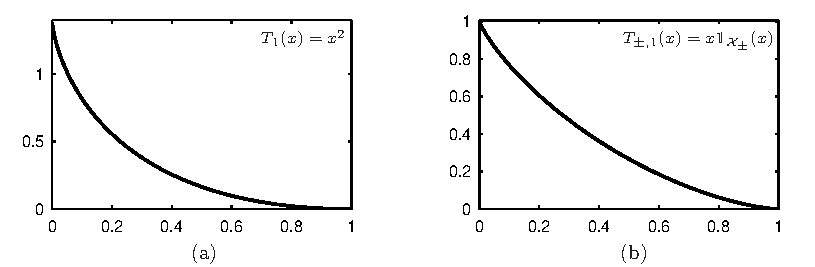
\includegraphics[width=.9\textwidth]{PDF/MaxEnt_LogisticLaw}}
\caption{Entropy  functional  $\phi_{\mathrm{u}}$   derived  from  the  logistic
  distribution:  (a)~with  $T_1(x)  =   x^2$  and  (b)~with  $T_{\pm,1}(x)  =  x
  \un_{\X_\pm}(x)$.}
%    ($c = \lambda_0 = 0, \lambda_1 = \overline{\lambda}_1 = -1$).}
\label{fig:Entropy-logistic}
\end{figure}



% ---------- Arcsine

\subsection{The arcsine distribution}
\label{subsec:Arcsine}

The arcsine distribution is a special case of the beta distribution with $\alpha
= \beta  = \frac12$. We  consider here the  centered and scaled version  of this
distribution which writes
%
\[
f_X(x) = \frac{1}{\pi\sqrt{ 2 \, \sigma^2 - x^2}} \qquad \mbox{on} \qquad \X = (
- \sigma \sqrt2 \, ; \, \sigma \sqrt2).
\]
%
The inverse distributions $f_{X,\pm}^{-1}$ on $\X_-  = ( - \sigma \sqrt2 \, ; \,
0 )$ and $X_+ = [ 0 \, ; \, \sigma \sqrt2 )$ write then
%
\[
f_{X,\pm}^{-1}(y) = \pm \frac{\sqrt{2 \pi^2  \sigma^2 y^2 - 1}}{\pi y}, \qquad y
\ge \frac{1}{\pi \sigma \sqrt2}
\]


Let us  now consider again  either a second  order moment as the  constraint, or
(partial) first order moment(s).


% -- Arcsine - second order

\subsubsection{Second order moment}

When  the second order  moment $T_1(x)  = x^2$  is constrained,  one immediately
obtains
%
\[
\phi'(y)=\lambda_0 + \lambda_1\left(2\sigma^{2}-\frac{1}{\pi^{2}y^{2}}\right)
\]
%
The family of entropy functional is then 
%
\[
\phi(y)  = c  +  \left( \lambda_0  +  2 \sigma^2  \lambda_1 \right)  y  \, +  \,
\frac{\lambda_1}{\pi^2 y}
\]
%
which    drastically   simplifies    with    the   special choice
%
\[
c  = 0,  \qquad \lambda_0  = -  \frac{\alpha^2}{\pi^2} \qquad  \mbox{and} \qquad
\lambda_1 = \pi^2 \qquad \mbox{to} \qquad\phi(y) = \frac{1}{y}
\]
%
% function   that   can   then    be   defined   over   which   is   represented
% figure~\ref{fig:Entropy-arcsin-var} for $\sigma=1$.


% ---------- Arcsine first order

\subsubsection{(Partial) first-order moment(s)}

Since the  distribution does not share the  sense of variation of  $T_1(x) = x$,
either we turn out to consider it as an extremal distribution of an entropy that
is not concave, or as a maximum entropy when constraints are of the type
%
\[
T_{\pm,1}(x) = x \un_{\X_\pm}(x)
% \quad \mbox{over} \quad \X_- = \left( - \sigma \sqrt2 \, ; \, 0
%\right), \quad \mbox{and} \quad \X_+ = \left[ 0 \, ; \: \sigma \sqrt2 \right).
\]
%
now 
%
\[
\phi_\pm'(y) = \sqrt2 \pi \sigma \lambda_0 + \lambda_{\pm,1} \frac{\sqrt{2 \pi^2
    \sigma^2  y^2 -  1}}{y} \qquad  \mbox{or} \qquad  \widetilde{\phi}_\pm'(y) =
\lambda_0 \pm \lambda_1 \frac{\sqrt{2 \pi^2 \sigma^2 y^2 - 1}}{y}
\]
%
where  the  different  factors  and  the  sign  are  absorbed  in  the  factors
$\lambda_0, \lambda_{\pm,1}$. A judicious choice can be to impose
%
\[
\lambda_{-,1} = \lambda_{+,1} = \overline{\lambda}_1 > 0
\]
%
and the  same integration constant $c$  for each branch, leading  then either to
the family of (convex)  uniform of functions $\phi(y) = \phi_{\mathrm{u}}(\sqrt2
\pi \sigma y)$ with
%
\[
\phi_{\mathrm{u}}(y) = c \, + \,  \lambda_0 \, u \, + \, \overline{\lambda}_1 \,
\left( \sqrt{u^2  - 1}  \, + \,  \arctan\left( \frac{1}{\sqrt{u^2 -  1}} \right)
\right) \un_{\left[1 \, ; \, +\infty \right)}(y)
\]
%
or,  in  the  non-convex  case,   to  the  family  of  functions  with  branches
$\widetilde{\phi}_{\pm}(y) = \widetilde{\phi}_{\pm,\mathrm{u}}(\sqrt2 \pi \sigma
y)$,
%
\[
\widetilde{\phi}_{\pm,\mathrm{u}}(y) = c \, + \, \lambda_0 \, u \, \pm \, \left(
  \sqrt{u^2 - 1} \, +  \, \arctan\left( \frac{1}{\sqrt{u^2 - 1}} \right) \right)
\un_{\left[ 1 \, ; \, +\infty \right)}(y)
\]


The      uniform      function      $\phi_{\mathrm{u}}$      is      represented
figure~\ref{fig:Entropy-arcsin}  for the  special  choice $c  =  \lambda_0 =  0,
\overline{\lambda}_1 = 1$  (here again, for $c = \lambda_0 =  0, \lambda_1 = 1$,
$\widetilde{\phi}_\pm = \pm \phi$).  In  this case again, the symmetrical choice
for  $\lambda_{\pm,1}$  allows to  recover  the  symmetries  of the  probability
density, and thus to a uniform convex entropy functional in the first context.

\
 
\begin{figure}[htbp]
\centerline{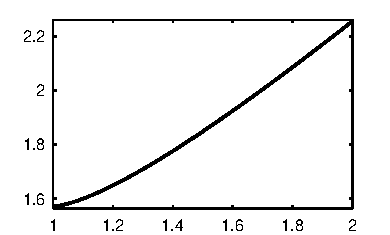
\includegraphics[width=.43\textwidth]{PDF/MaxEnt_ArcsineLaw}}
\caption{Entropy  functional   $\phi_{\mathrm{u}}$  derived  from   the  arcsine
  distribution with partial constraints $T_{\pm,1}(x) = x \un_{\X_\pm}(x)$.}
\label{fig:Entropy-arcsin}
\end{figure}


% ---------- Gamma first order

\subsection{The gamma distribution and (partial) $p$-order moment(s)}

\label{subsec:GammaFirstOrder}

As a very special case, consider here this distribution, expressed
as
%
\[
f_X(x) = \frac{\beta^\alpha  x^{\alpha-1} \exp(-\beta x)}{\Gamma(\alpha)} \qquad
\mbox{on} \qquad \X = \Rset_+.
\]
%
Let  us concentrate  on the  case $\alpha  > 1$  for which  the  distribution is
non-monotonous, unimodal, where the mode is located at $x = x_{\mathrm{m}}$, and
$f_X(\Rset_+) = \left[ 0 \, ; \, \frac1{\tau \,e^{\alpha-1}} \right]$ with
%
\[
x_{\mathrm{m}}  =   \frac{\alpha-1}{\beta}  \qquad  \mbox{and}   \qquad  \tau  =
\frac{\Gamma(\alpha)}{\beta \, (\alpha-1)^{\alpha-1}}
\]
%
Thus, here again it cannot be  viewed as a maximum entropy constraint neither by
any $p$-order  moment.  Here,  we can  again interpret it  as a  maximum entropy
constrained by partial moments
%
\[
T_{k,1}(x) = x^p, \quad k \in \{ 0  , -1 \} \qquad \mbox{over} \qquad \X_0 = [ 0
\, ; \, x_{\mathrm{m}} ) \qquad  \mbox{and} \qquad \X_{-1} = [ x_{\mathrm{m}} \,
; \: +\infty ).
\]
%
or as an extremal entropy constrained by the moment 
%
\[
T_1(x) = x^p \quad \mbox{over} \quad \X = \Rset_+
\]
%
where $p > 0$. Inverting $y = f_X(x)$ leads to the equation
%
\[
-  \frac{x}{x_{\mathrm{m}}} \exp\left(  - \frac{x}{x_{\mathrm{m}}}  \right)  = -
(\tau  \,  y )^{\frac{1}{\alpha -  1}}
%  \qquad  \mbox{with}  \qquad \tau  =  \left(
%  \frac{\Gamma(\alpha)}{\beta                              (\alpha-1)^{\alpha-1}}
%\right)^{\frac{1}{\alpha-1}}
\]
%
to be solved. As expected, this equation has two solutions. These
solutions can be expressed via the multivalued Lambert-W function
$\W$ defined by $z=\W(z)\exp(\W(z))$, leading to the inverse functions
\[
f_{X,k}^{-1}(y) = - x_{\mathrm{m}}  \, \W_k\left( - (\tau y)^{\frac{1}{\alpha
      - 1}} \right), \qquad y \in \left[ 0 \, ; \, \frac{1}{\tau e^{\alpha - 1}}
\right],
\]
%
where  $k$  denotes  the branch  of  the  Lambert-W  function. $k=0$  gives  the
principal branch and here it is related  to the entropy part on $\X_0$, while $k
= -1$ gives the secondary branch, related to $\X_{-1}$ here.

One has thus to solve the equation
%
\[
\phi'_k(y) =  \lambda_0 \tau  + \lambda_{k,1} \tau  \left[ - \W_k\left(  - (\tau
    y)^{\frac{1}{\alpha - 1}} \right) \right]^p
\]
%
where the  positive factor  are absorbed in  the $\lambda_0,  \lambda_{k,1}$ and
where to insure the convexity of the $\phi_k$,
%
\[
(-1)^k \lambda_{k,1} > 0
\]
%
The  same  approach  allows   to  design  $\widetilde{\phi}_k$,  with  a  unique
$\lambda_1$ instead of the $\lambda_{k,1}$.  Integrating the previous expression
is not an  easy task. Noting that $\W_k'(x)  = \frac{\W_k(x)}{x (1+\W_k(x))}$, a
way to make  the integration is to search  $\phi_k(y) = \phi_{k,\mathrm{u}}(\tau
y)$  where $\phi_{k,\mathrm{u}}(u)$  is searched  as the  product of  $u \left[-
  \W_k\left(  -  u^{\frac{1}{\alpha-1}} \right)  \right]^p  $  and  a series  of
$\left[  - \W_k\left(  -  u^{\frac{1}{\alpha-1}} \right)  \right]$  and then  to
recognize the coefficients  of the series. Such an approach  leads to the family
of entropic functional $\phi_k(y) = \phi_{k,\mathrm{u}}(\tau y)$ with
%
\[\begin{array}{l}
\phi_{k,\mathrm{u}}(u) \: = \: c_k + \lambda_0 \, u\\[2mm]
%
\hspace{7.5mm} + \, \lambda_{k,1} \, u \left[ - \W_k\left(
    -   u^{\frac{1}{\alpha-1}}   \right)  \right]^p   \left[   1  -
  \frac{p}{p+\alpha-1} \,  \, \hypgeom{1}{1}\left(  1 \, ;  \, p+\alpha \,  ; \,
    (1-\alpha)  \W_k   \left(  -  u^{\frac{1}{\alpha-1}}  \right)
  \right) \right] \un_{\left[ 0 \, ; \, e^{1-\alpha} \right]}(u)
\end{array}\]
%
where $\hypgeom{1}{1}$  is the  confluent hypergeometric (or  Kummer's) function
and  $c_k$ are  integration  constants. The integration constant
% (the  positive  multiplicative factor  is
%absorbed in the $\lambda_{k,1}$).  $\X_{-1}$ being unbounded, $c_{-1}$ is chosen
%to  be zero  and  $c_0$ 
can be chosen such that $\phi_k$ coincide in 0 for instance, that gives
%
\[
%c_0 = 0 \qquad \mbox{and} \qquad  
c_{-1} - c_0 \,  = \, \frac{p \, \Gamma(p+\alpha-1)}{(\alpha-1)^{p+\alpha-1}} \,
\lambda_{-1,1}
\]
%
(see~\cite[eq.~13.1.4]{AbrSte70} and \cite[eq.]{CorGon96}).   The same algebra leads to
the same  expression for  the $\widetilde{\phi}_k$, except  that $\lambda_{k,1}$
are replaced by a unique $\lambda_1$.

The  multivalued   function  $\phi_{\mathrm{u}}$  in  the   concave  context  is
represented figure~\ref{fig:Entropy-gamma} for $p = 2, \alpha = 2$ and $\alpha =
5$,  and  with  the  choices  $c_{-1}  =  \lambda_0  =  0,  \lambda_{0,1}  =  1,
\lambda_{-1,1} = - 0.1$.
%
\begin{figure}[htbp]
\centerline{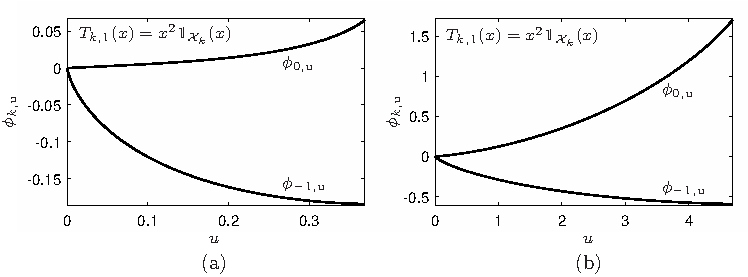
\includegraphics[width=.9\textwidth]{PDF/MaxEnt_GammaLaw}}
\caption{Multiform entropy functional $\phi_{\mathrm{u}}$ derived from the gamma
  distribution   with  the   partial  moment   constraints  $T_{k,1}(x)   =  x^2
  \un_{\X_k}(x)$, $k\in\{0,-1\}$.  (a): $\alpha = 2$; (b): $\alpha = 5$.}
%
\label{fig:Entropy-gamma} 
\end{figure}

\bibliographystyle{unsrt}
\bibliography{New_entropies}
\end{document}
